\chapter{Návrh}\label{chap:design}

V této kapitole se budu věnovat návrhu knihovny na automatizaci a jejím funkčním požadavkům.

\section{Účastníci testování}\label{sec:participants}
V rámci knihovny a testovacího běhu se bude vyskytovat několik účastníků testování. Mezi účastníky testování bude patřit:

\begin{description}
    \item[Testovací služba] Služba, která řídí testovací běh.
    \item[Testované zařízení] Hlavní účastník testování, který běží na jiném zařízení, než ze kterého běží testovací služba. 
    \item[Testovací partner] Zařízení, které simuluje nějaké testovaného zařízení. Toto zařízení běží na stejném zařízení, jako testovací služba. 
\end{description}

Testovací služba bude jádrem k řízení testování. Tato služba poběží na samostatném zařízení, které bude běžet na operačním systému Windows. Zařízení bude v rámci infrastruktury serveru Azure DevOps agent. Testovací služba bude implementována v jazyce \csharp{}. Všechna implementace v jazyce \csharp{} bude vytvořena pro .NET Framework 4.8. 

Hlavním cílem je testovat vyvíjený produkt. Toto zařízení v rámci knihovny bude bráno jako testované zařízení. Testovací služba bude podporovat připojení jednoho a více testovaných zařízení a při každém testovacím běhu musí být připojeno alespoň jedno testovací zařízení. Tato zařízení budou připojeno k zařízení, ze kterého poběží testovací služba, za pomocí Ethernet připojení. Zařízení SIMATIC ET 200SP má svojí implementaci v jazyce \cpp{}. Z toho vyplývá že implementace pro toto zařízení bude vytvořena v tomto jazyce. 

Součástí knihovny zároveň bude také tzv. testovací partner. Tento účastník slouží k simulaci testovaného zařízení, buď jako celku, nebo pouze nějaké jeho činnosti. Zařízení může simulovat zařízení jako PLC, nebo různé nástroje, které slouží například k certifikaci zařízení. Simulováním zařízení snižujeme hardwarové nároky na testování, což vede ke snížení ekonomických nákladů na testování. Tato zařízení se budou připojovat v závislosti na jednotlivých testech. Následně po skončení testu budou tato zařízení odpojena. Testovací zařízení bude stejně jako testovací služba vytvořeno v jazyce \csharp{}.

Maximální počet připojených zařízení ke službě se odvíjí od limitací protokolu TCP/IP a jeho implementace v jazyku \csharp{}. Tento limit se ale pohybuje ve stovkách, v kontrastu očekávaný počet zároveň připojených zařízení se bude pohybovat v desítkách. Tedy tento limit knihovnu v ničem neomezuje.

Účastníky testování a jejich propojení můžeme vidět znázorněné na obrázku \ref{fig:devicemodel}. Na tomto obrázku můžeme vidět agenta, resp. zařízení na kterém poběží testovací služba a případní testovací partneři, primární testované zařízení SIMATIC ET 200SP a PLC. PLC zařízení značí jakékoliv zařízení, které není simulováno knihovnou.

\begin{figure}[htbp]
    \centering 
    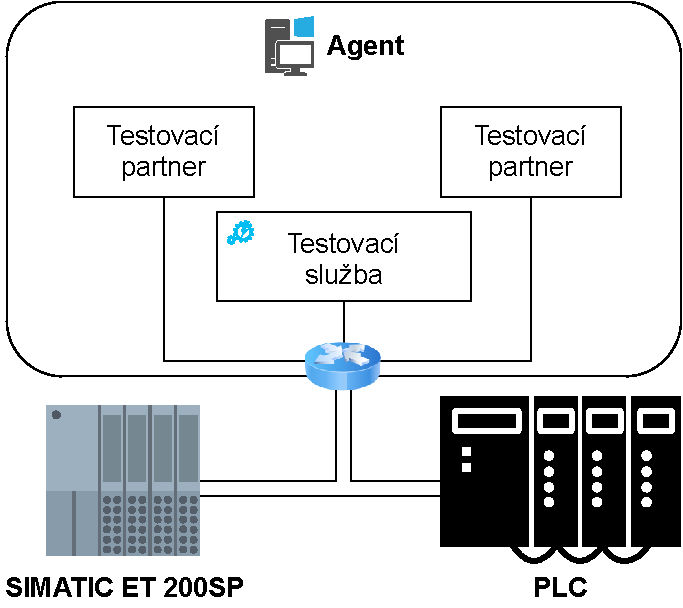
\includegraphics[width=0.7\textwidth]{assets/img/devicemodel.pdf}
    \caption{Propojení účastníků testování}
    \label{fig:devicemodel}
\end{figure}

\section{Komunikace}
Komunikace mezi všemi účastníky testování bude fungovat na principu TCP/IP připojení. Testovací služba a zařízení, na kterém služba poběží, bude sloužit jako server a všichni účastnící testovaní budou klienti, kteří se budou k tomuto zařízení připojovat. 

Jednotlivé zprávy, které budou mezi testovací službou a všemi účastníky testování vyměňovány, budou mít jasně stanovenou strukturu. Diagram složení zprávy lze vidět na obrázku \ref{fig:message}. Na tomto obrázku můžeme vidět, že jedna zpráva lze rozdělit na dvě části -- hlavičku zprávy a data zprávy. Zároveň jak můžeme vidět, jedna buňka v diagramu odpovídá jednomu bajtu. 

\begin{figure}[htbp]
    \centering 
    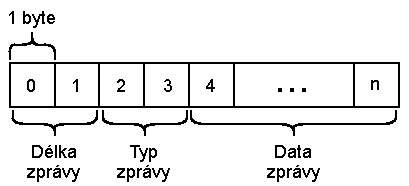
\includegraphics{assets/img/message.pdf}
    \caption{Diagram struktury jedné zprávy}
    \label{fig:message}
\end{figure}

Zpráva bude obsahovat povinně hlavičku zprávy. Tato hlavička bude obsahovat typ zprávy a délku dat zprávy. Jak můžeme vidět na diagramu, každý z těchto údajů bude mít velikost dva bajty. Celkově tedy hlavička bude o velikosti 4 bajty. Knihovna bude podporovat tyto typy zpráv:

\begin{enumerate}
    \item \inlinecode{MSG\_OK} -- Zpráva o úspěchu/potvrzení
    \item \inlinecode{MSG\_FAIL} -- Zpráva o neúspěchu
    \item \inlinecode{MSG\_TEST} -- Direktiva ke spuštění testu
    \item \inlinecode{MSG\_STOP} -- Direktiva k ukončení testování
\end{enumerate}

Za hlavičkou zprávy následně budou moct být uložena data zprávy. Tyto data avšak budou nepovinná. V těchto případech, kdy zpráva nebude neobsahovat data zprávy, bude pro přenesení informace postačovat pouze typ zprávy a v hlavičce bude uvedena nulová hodnota jako délka dat zprávy. 

Maximální délka jedné zprávy se bude odvíjet od limitací použitých technologií. Limit se bude primárně odvíjet od Ethernet protokolu, který podporuje nejmenší maximální délku jednoho packetu ze všech použitých protokolů, a to 1500 bajtů. Toto číslo avšak také zahrnuje všechny potřebné hlavičky k přenosu packetu. Proto jako maximální délka jedné zprávy bude zvolena délka 1400 bajtů. Toto číslo ponechává místo pro potřebné hlavičky a zároveň je více než dostatečné pro navrhované použití. \cite{max_packet_size} 

Všechny hodnoty zprávy budou ukládány v kladné (anglicky tzv. unsigned) podobě. Jedinou kontrolní informací, kterou bude zpráva obsahovat, je délka dat zprávy. Protokol TCP/IP avšak sám obsahuje jednoduchou detekci chyb. Všechny tyto kontroly budou považovány jako dostatečné.

Účastníci testování se na začátku připojí k testovací službě a odešlou inicializační zprávu. Tato zpráva bude typu 1 a v datech zprávy bude obsahovat svojí MAC adresu. Výjimkou budou testovací partneři, kteří budou jako svoji MAC adresu odesílat adresu \inlinecode{DE:AD:BE:EF:00:00}. Díky tomu je testovací služba jednoduše identifikuje. Testovací služba následně odešle potvrzovací zprávu o úspěšném připojení s typem 1, bez žádných dat. V případě vzniku chyby služba odešle zprávu typu 2, bez dat. 

Pro započnutí testování a spuštění jednotlivých stádií testování služba odešle všem účastníkům testování zprávu s typem 3. V datech zprávy služba odesílá tyto data:

\begin{enumerate}
    \item Číselnou reprezentaci identifikátoru testu. Ten je uložen v prvních 4 bajtech dat zprávy.
    \item Číselnou reprezentaci identifikátoru, který určuje fázi testu. Uložen je ve dvou bajtech dat zprávy hned za identifikátorem testu. Fáze testování jsou blíže popsány v sekci \ref{sec:test_run}.
\end{enumerate}

Služba následně čeká na odpověď od všech účastníků testování. Účastnící odesílají testovací službě po skončení testovacího stádia zprávu bez dat, s typem 1 v případě úspěchu a s typem 2 v případě neúspěchu. Po skončení testování služba odesílá všem účastníkům testování zprávu s typem 4, bez žádných dat. 

Ukázku komunikace můžeme vidět znázorněnou na sekvenčním diagramu, který je na obrázku \ref{fig:seqdiag}. Na tomto sekvenčním diagramu můžeme vidět výměnu zpráv mezi testovací službou a dvěma účastníky testování během spuštění jednoho testu. Direktiva \inlinecode{Message} znázorňuje jednu zprávu, kde v závorkách můžeme vidět nejdříve typ zprávy a následně data zprávy (pokud zpráva nějaká data obsahuje). V diagramu zároveň můžeme vidět využití testovacího partnera.

\begin{figure}[htbp]
    \centering 
    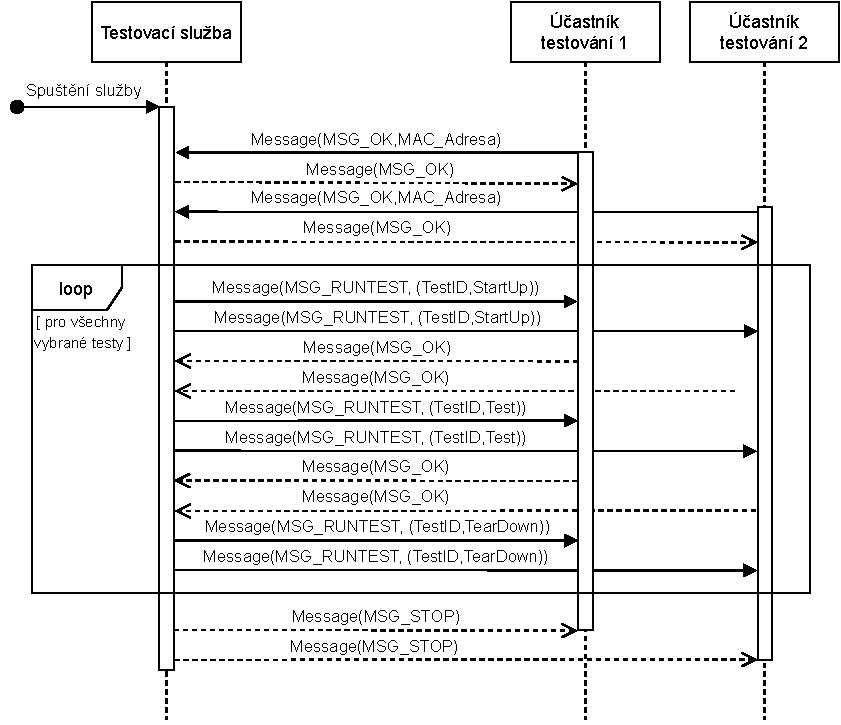
\includegraphics[width=0.95\textwidth]{assets/img/sequencediagram.pdf}
    \caption{Sekvenční diagram znázorňující běh služby}
    \label{fig:seqdiag}
\end{figure}

\section{Testovací služba}
Jak jsem již zmínil v sekci \ref{sec:participants}, testovací služba bude jádrem celého testování. Tato služba bude řídit celý testovací běh a předávat všem účastníkům testování pokyny. Zároveň bude synchronizovat testovací běh mezi všemi účastníky testování. Běh služby můžeme vidět znázorněný na stavovém diagramu, které je znázorněn na obrázku \ref{fig:statediag}. Jednotlivé stavy jsou vysvětleny v následujících sekcích. 

\begin{figure}[htbp]
    \centering 
    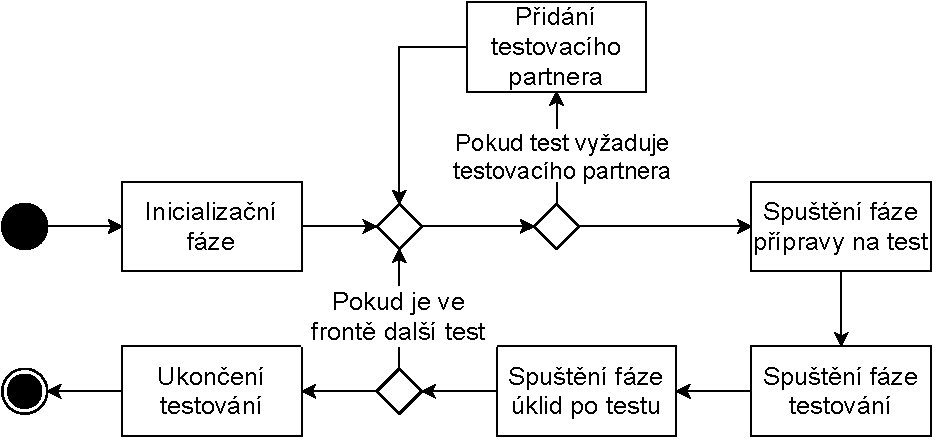
\includegraphics[width=0.75\textwidth]{assets/img/servicestatediagram.pdf}
    \caption{Stavový diagram služby}
    \label{fig:statediag}
\end{figure}

\subsection{Inicializace služby}
Testovací služba započíná běh inicializační fází. Služba v inicializační fázi vytvoří připojení se všemi testovanými zařízeními, dle nadefinované komunikace. Z konfigurace služba bude vědět, kolik testovaných zařízení má očekávat. Inicializační fáze zároveň bude mít definovaný časový limit, který ve výchozí konfiguraci bude 60 sekund. Zároveň ale bude nastavitelný uživatelem. Testovací služba vyhodnotí inicializační fázi jako úspěšnou, pokud se úspěšně připojí definovaný počet testovaných zařízení. Služba vyhodnocuje neúspěch inicializační fáze v případě že nastanou tyto situace:

\begin{itemize}
    \item vypršení časového limitu na inicializační fázi
    \item chyba v komunikaci, nesprávná komunikace
    \item nepřipojení definovaného počtu zařízení
    \item připojení testovacího partnera
\end{itemize}

V případě neúspěchu inicializační fáze služba nastavuje stav služby jako chybný. Testy poté nebudou provedeny.

\subsection{Spravování testovacích partnerů}
Služba bude podporovat připojení testovacích partnerů. Tato zařízení se budou připojovat před spuštěním jednotlivých testů. Testovací služba obdrží direktivu k očekávaní připojení testovacího partnera. Partner následně projde stejnou inicializační fází jako ostatní testovaná zařízení. Služba vyhodnocuje neúspěch připojení testovacího partnera v těchto případech:

\begin{itemize}
    \item připojení jiného zařízení, než testovacího partnera
    \item vypršení časového limitu na připojení
    \item chyba v komunikaci
\end{itemize}

V opačném případě služba vyhodnocuje úspěch. Po dokončení testu služba odesílá všem připojeným partnerům direktivu k ukončení testování a ukončuje spojení s nimi. 

\subsection{Registrování testů}
Testovací služba nebude mít žádné informace o jednotlivých testech. Jedinou informaci, kterou testovací služba obdrží, bude číselný identifikátor testu. Reprezentace testů čísel může způsobit kolizi mezi testovými identifikátory. Služba samotná tuto kolizi kontrolovat nebude. Způsob detekce kolize je popsán v sekci \ref{sec:reg_test}.

\subsection{Testovací běh}\label{sec:test_run}
Po úspěšné inicializační fázi a případném připojení testovacích partnerů služba čeká na direktivu ke spuštění testu. Po obdržení této direktivy s identifikátorem testu služba odesílá všem účastníkům testování zprávu k zahájení první fáze testu. Tuto fázi budeme označovat jako přípravu na testování. V této fázi účastníci testovaní připraví všechny potřebné prostředky pro provedení testu. Účastníci následně odesílají zprávu o úspěchu/neúspěchu této fáze. Služba vyhodnocuje fázi jako úspěšnou pokud od všech účastníků obdrží zprávu o úspěchu. V opačném případě vyhodnocuje fázi jako neúspěšnou.

Služba po vyhodnocení úspěchu první fáze přechází do fáze druhé. V této fázi proběhne samotné testování. Služba odešle všem účastníkům zprávu ke spuštění této fáze. Následně očekává odpověď od všech účastníků. Služba, stejně jako v předchozí fázi, vyhodnocuje fázi jako úspěšnou, pokud obdrží zprávu o úspěchu od všech účastníků testování. V opačném případě je neúspěšná.

Poslední fází testu je úklid po testu. V této fázi služba opět vyšle zprávu k započetí fáze. Účastníci testování v této fázi uvádějí zařízení do stavu, ve kterém bylo před zahájením testu. Následně účastníci odešlou zprávu o úspěchu/neúspěchu. Vyhodnocení úspěchu/neúspěchu je stejné jako v předchozích fázích.

Po odeslání zprávy s direktivou k spuštění jednotlivých fází testu služba čeká, než obdrží odpověď od všech účastníků testu. Tyto body, kdy služba čeká na odpověď od všech účastníků testu, budeme nazývat synchronizační body. Účastníci, kteří dokončili svojí fázi testu, čekají na direktivu od testovací služby. Tímto se běh synchronizuje mezi všemi účastníky testu. Jednoduše lze odvodit, že během jednoho testu nastávají tři synchronizační body. 

Tyto synchronizační body budou mít definovaný časový limit. Při spuštění testu tester bude moct zadat vlastní časový limit, který bude použit po každé z fází. Tedy tester bude zadávat předpokládaný maximální časový limit nejdelší fáze testování. Zároveň je ale potřeba vzít v úvahu, že časový limit je spuštěn ihned po odeslání všech zpráv. Tento časový limit bude ve výchozí konfiguraci opět 60 sekund. 

Testovaná zařízení se v době běhu testu mohou dostat do chybového stavu, ve kterém nebude možné pokračovat v testování. Testovací služba tedy bude předpokládat tyto chybné stavy:


\begin{description}
    \item[Nezajištění konzistence testování] Pro konzistenci testů testovací služba vyžaduje, aby po každém testu testované zařízení bylo ve stejném stavu jako bylo před začátkem testu. Pokud účastník testu odešle neúspěch ve fázi přípravy na test, nebo ve fázi úklidu po testu, tak poté bude tento účastník považován jako chybném stavu. V případě že chyba nastane ve fázi přípravy na test, služba neprovádí fázi testování a přechází do fáze úklidu po testu. 
    \item[Vypršení časového limitu] Vypršení časového limitu primárně znamená, že služba ve stanové době neobdržela odpověď od účastníka testování, ale tento účastník je stále připojen k testovací službě. Toto vede k závěru, že tento účastník je v chybovém stavu a další testování není možné. 
    \item[Chyba v komunikaci] Pokud během testu zařízení odpoví jinak, než dle stanovené komunikace, tak poté bude toto zařízení považováno jako v chybném stavu. Zároveň bude za chybu považováno odpojení zařízení od služby.  
\end{description}

Pokud všechny fáze testu byli úspěšné, tak poté služba vyhodnocuje test jako úspěšný. Obráceně služba vyhodnocuje test jako neúspěšný pokud jedna z fází byla neúspěšná. V případě nastání chyby, kde testované zařízení je předpokládáno jako v chybovém stavu, testovací služba nastavuje svůj stav jako chybový. Následující testy nebudou provedeny.


\subsection{Ukončení testování}
Testovací služba po obdržení direktivy k ukončení služby odesílá všem připojeným účastníkům testování zprávu k ukončení testovacího běhu. I když služba může některého z účastníků považovat jako v chybném stavu, pokud je tento účastník stále ke službě připojen, tak poté mu služba odešle tuto ukončovací zprávu. Toto se děje s cílem úspěšně ukončit co nejvíce zařízení.


\section{Rozhraní pro testování}
Důležitou součástí knihovny budou rozhraní, které umožní implementaci propojení s testovací službou a tím samotné testování. Knihovna bude obsahovat dvě důležitá rozhraní. 

\subsection{Rozhraní testu}
Jak jsem již popsal v sekci \ref{sec:test_run}, jednotlivé testy budou mít tři fáze testování:

\begin{enumerate}
    \item Příprava na testování -- definování potřebných struktur, inicializace
    \item Testování -- provedení samotného testu
    \item Úklid po testu -- uvolnění využitých zdrojů
\end{enumerate}

Testovací knihovna tedy bude definovat rozhraní, které bude vyžadovat, aby tyto tři fáze testu byli pro každý test definované. Návrh rozhraní můžeme vidět na výpisu \ref{listing:test_if}. Na tomto výpisu můžeme vidět, že každé fázi odpovídá jedna metoda. Tyto metody následně vrací jednoduchou informaci o úspěchu/neúspěchu. To znamená, že vyhodnocení jednotlivých fází bude na jednotlivých testerech a jejich implementaci. Jednotlivé komponenty knihovny pouze obdrží informaci o výsledku fáze.

\begin{listing}[htbp]
    \begin{minted}[breaklines]{text}
    ITestCase 
    {
        bool StartUp()

        bool Test()

        bool TearDown()
    }
    \end{minted}
\caption{Návrh rozhraní pro jeden test}
\label{listing:test_if}
\end{listing}



\subsection{Rozhraní pro testované zařízení}

Dalším důležitým rozhraním bude rozhraní pro testované zařízení. Toto rozhraní bude definovat metody, které bude potřeba definovat na každém testovaném zařízení. Cílem je, aby toto rozhraní bylo co nejjednodušší pro co nejrychlejší implementaci na nově testovaném zařízení.

Návrh tohoto rozhraní můžeme vidět na výpisu \ref{listing:dev_if_abstract}. Jak můžeme z výpisu vidět vidět, první tři metody se starají o propojení s testovací službou. Metoda \inlinecode{createConnection} bude implementovat vytvoření propojení s testovací službou. Metoda pouze vytvoří propojení s testovací službou na základě TCP/IP protokolu a následně vrátí informaci o úspěšnosti. Cíl připojení, tedy IP adresu a port na kterém poběží testovací služba, metoda obdrží v argumentech.

O samotné odesílání, resp. přijímání jednotlivých zpráv se bude starat metoda \inlinecode{sendMessage}, resp. \inlinecode{rcvMessage}. Metoda \inlinecode{sendMessage} po svém zavolání převede objekt zprávy, obdržený v argumentu metody, na bajtové pole, které následně odešle testovací službě. Metoda \inlinecode{rcvMessage} symetricky zprávu od testovací služby přijme a převede ji na objekt jedné zprávy. Následně odkaz na tuto zprávu uloží do argumentu, který je výstupní. Obě tyto metody vrací informaci o úspěchu/neúspěchu.

Metoda \inlinecode{getTest} bude určena k získání jednotlivých instancí testů. Testy, které bude tato metoda vracet, musí být dle dříve nadefinovaného rozhraní pro jednotlivé testy. Metoda obdrží číselnou reprezentaci testu a na základě toho poté vrátí správnou instanci testu. 

Metoda \inlinecode{getMacAddress} bude, jak již z názvu vyplývá, vracet MAC adresu zařízení. V neposlední řadě metoda \inlinecode{print} bude sloužit k výpisu průběhu běhu. Tento výpis by měl hlavně posloužit k náhledu na průběh testovacího běhu, pokud se během běhu vyskytnou například nějaké chyby.

\begin{listing}[htbp]
    \begin{minted}[breaklines]{text}
    ITestClient 
    {

        bool createConnection(ipAddress, port)

        bool sendMessage(message)

        bool rcvMessage(message)

        ITestCase getTest(test)

        void print(toPrint)

        bool getMacAddress(macAddr)
    
    }
    \end{minted}
\caption{Ukázka definice rozhraní}
\label{listing:dev_if_abstract}
\end{listing}

\section{Běh testovaného zařízení}

O samotný běh jednotlivého testovaného zařízení se bude starat samostatná komponenta, která bude nezávislá na jakémkoliv zařízení. Tato komponenta se bude nazývat v knihovně tzv. \inlinecode{TestRunner}.

Komponenta bude obsahovat veškerou logiku testovacího běhu pro jednotlivé testované zařízení. Při zahájení testování komponenta za pomocí rozhraní vytvoří propojení s testovací službou a odešle zprávu o úspěchu, kde v datech zprávy uvede svoji MAC adresu. Po obdržení zprávy o úspěchu od testovací služby komponenta přechází do metody, která bude obsluhovat příchozí zprávy. 

Komponenta bude očekávat dva typy zpráv - direktivu ke spuštění testu a direktivu k ukončení testování. Po obdržení direktivy k započetí testu, komponenta ze zprávy zjistí identifikátor testu a testovací fázi. Následně z rozhraní získá instanci testu, který si po dobu běhu testu drží. Poté dle instrukcí spouští jednotlivé fáze testování. Po konci každé testovací fáze komponenta odesílá zprávu o úspěchu/neúspěchu testovací službě.

Dle této implementace může teoreticky dojít k tomu, že testované zařízení obdrží zprávu s požadavkem na spuštění fáze testování nebo fáze úklidu po testu, ještě předtím, než obdrží instrukci ke spuštění fáze přípravy na test. Komponenta tuto situaci kontroluje a v případě jejího vzniku automaticky odesílá zprávu o neúspěchu fáze. 

Průběh testovacího běhu testovaného zařízení lze vidět na diagramu aktivit, který můžeme vidět na obrázku \ref{fig:act_diag_device}. Jak lze z diagramu vidět, běh zařízení se silně odvíjí od příkazů, které obdrží od testovací služby. Zároveň na diagramu můžeme vidět již zmíněné tři synchronizační body. Tyto body jsou zvýrazněny modrým čárkovaným obdélníkem. Z diagramu se může zdát, že pokud zařízení ve fázi přípravy na testování nebo ve fázi úklidu po testu vrátí neúspěch, tak poté lze pokračovat v testování. Toto ale není pravda, protože tento případ testovací služba nepovolí a po dokončení tohoto testu, který způsobil danou chybu, bude testovací běh ukončen. Výjimkou jsou pouze testovací partneři. Tyto zařízení jsou po konci testu ukončována, proto jejich chybný stav nemá následky na další testy.

\begin{figure}
    \centering 
    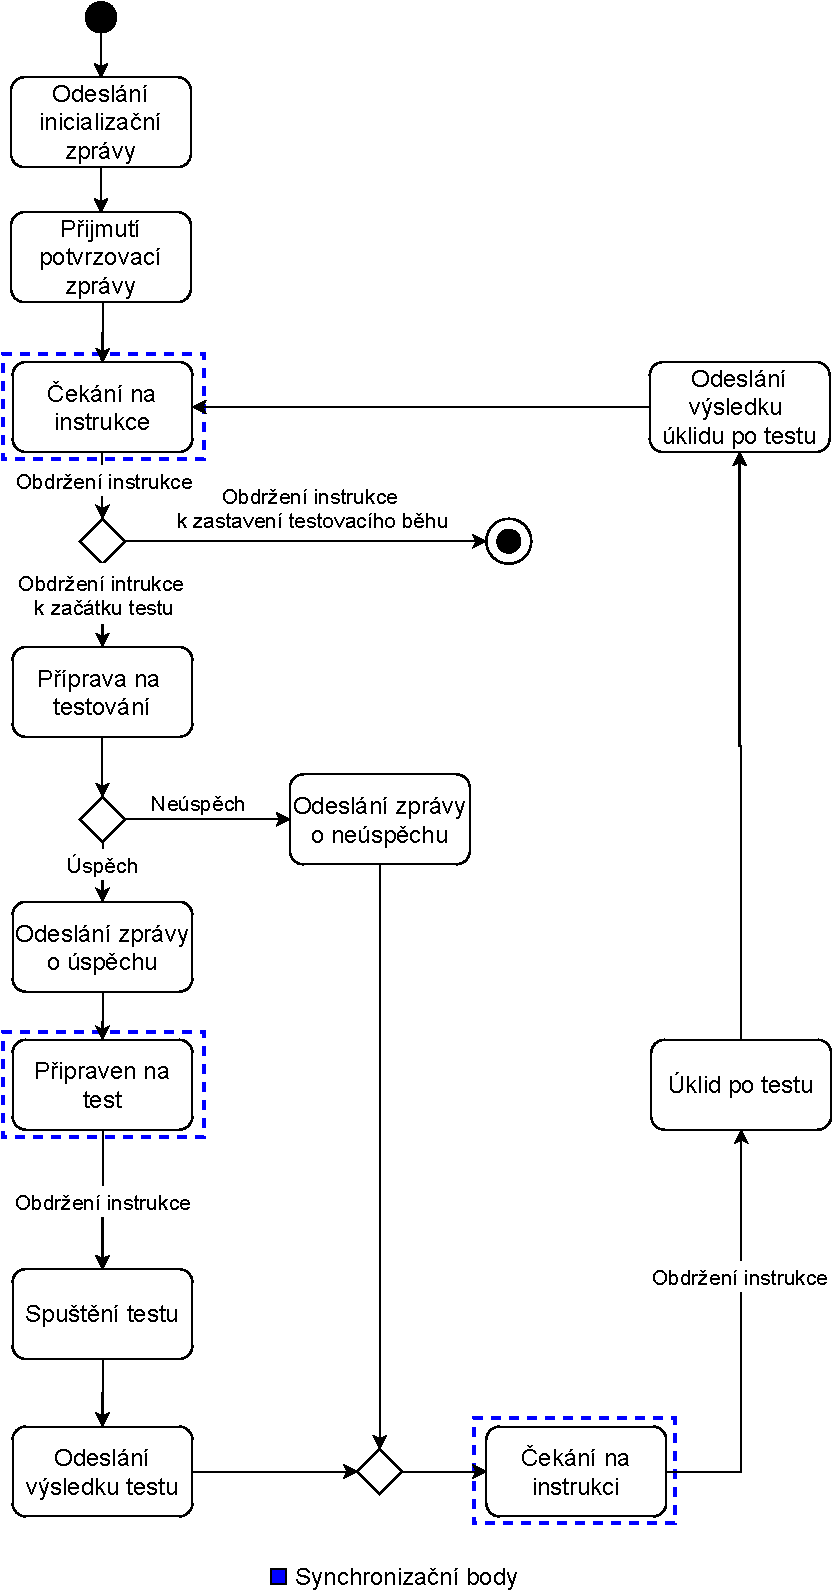
\includegraphics[height=0.98\textheight]{assets/img/activitydiagramdevice.pdf}
    \caption{Diagram aktivit testovaného zařízení}
    \label{fig:act_diag_device}
\end{figure}


\section{Testovací partner}
Testovací partner je speciálním druhem účastníka. Toto zařízení bude spouštěno ze stejného zařízení, jako testovací služba. Zařízení bude fungovat primárně na stejném principu, jako testovaná zařízení. Tedy, zařízení bude mít implementované rozhraní pro testované zařízení, které bude ovládáno komponentou \inlinecode{TestRunner}. 

Změnou je způsob ovládání této komponenty. Komponenta bude zaobalena vlastní třídou, která tuto komponentu bude spouštět na vlastním vlákně. Toto bude umožňovat nezávislý běh zařízení. Rozdílem také bude způsob definování testů. Testovací partner bude podporovat dva typy způsobů jak definovat testy. První způsobem bude za pomocí předání jedné instance testu. Jelikož testovací partner je vázán na jednotlivé testy, je tento přístup nejjednodušší. Dalším způsobem bude předání funkce, která bude vracet instance testů na základě číselného identifikátoru. Tento způsob je totožný jako u testovaných zařízení a v určitých případech může usnadnit správu těchto zařízení. 

Testovací partner bude spouštěn z testovacího projektu za pomoci testovací knihovny. Vytvořená instance partnera bude předána testovací knihovně, která se následovně postará o jeho spuštění a ukončení. Zařízení bude po konci testu odpojeno od testovací služby. Testovací knihovna bude kontrolovat úspešnost tohoto ukončení a v případě neúspěchu standardního ukončení testovací knihovna ukončí vlákno, na kterém zařízení poběží.

Testovací služba nebude nijak omezovat maximální možný počet připojených testovacích partnerů. Jediné omezení, které teoreticky může vzniknout, bude v případě, že při vytváření vláken pro jednotlivá zařízení se vyčerpá maximální počet dostupných vláken. Toto by ale při reálném použití neměl být problém, jelikož je předpokládáno, že počet těchto zařízení využitých pro jeden test se bude pohybovat maximálně v desítkách. 


\section{Propojení se serverem Azure DevOps}

Jedním z cílů této práce je vytvoření takového připojení, aby server Azure DevOps byl schopen spouštět jednotlivé testy a zároveň obdržel výsledek testu. K tomuto propojení využijeme testovací framework MSTest, který je nativně podporovaný serverem Azure DevOps. Celé následující propojení je možné díky uložení projektu v Azure Repos.

\subsection{Propojení s frameworkem MSTest}
Cílem vytvořeného propojení je, aby bylo co nejvíce automatizované a obsahovalo co nejméně práce ze strany testera. MSTest bude nezávisle na jednotlivých testech inicializovat službu před započnutím testování. V této době proběhne inicializační fáze služby. 

Následně framework MSTest bude spouštět jednotlivé vybrané testy. V testech bude zadávat testovací službě direktivu ke spuštění testu. Zároveň bude moct před zavoláním direktivy přidávat jednotlivé testovací partnery. Následně po skončení testu framework MSTest vyhodnotí úspěšnost testu.

Po proběhnutí jednotlivých testů framework MSTest službu ukončuje. V případě vzniku chyby během testování, díky které nebude možné pokračovat v testování, bude framework vyhodnocovat tyto testy jako bezvýsledné a testy přeskočí.

Propojení testovací služby a testovacího frameworku MSTest bude zajišťovat API. Toto API bude určovat přístupné metody, které mohou být využity v testovacím frameworku. Zároveň bude jedinou komponentou, kde bude framework MSTest v knihovně využívat.

\subsection{Registrování testů}\label{sec:reg_test}
Registrování testů ve frameworku MSTest a testovací službě bude na sobě nezávislé. Framework MSTest automaticky objevuje metody, které jsou označeny jako testovací. Framework MSTest v implementaci pro jazyk \csharp{} využívá pro rozlišení testovacích součástí tzv. atributy. Atributy přidávají metadata k třídám, typům, metodám atd. \cite{attribute_docs}. Testovací knihovna bude rozšiřovat tyto atributy o atribut \inlinecode{TestEnum}. Tento atribut bude identifikovat typy enumerátorů, které reprezentují testy. 

Tím, že testovací služba může přijmout jakýkoliv enumerátor, tak může vzniknout kolize mezi jednotlivými typy enumerátorů. V inicializační fázi proto bude API kontrolovat, zda enumerátory s atributem \inlinecode{TestEnum} neobsahují mezi sebou neobsahují kolizi a v případě jejího vzniku vyhodí výjimku a nepokračuje v testování.

Jednotlivé testy frameworku MSTest následně budou registrovány na serveru Azure DevOps. Na serveru Azure DevOps tester vytvoří tzv. Test Case, který následně asociuje odpovídající testovací metodě frameworku MSTest. Vytvoření této asociace je nativně podporované v IDE Visual Studiu, ve kterém je celá knihovna vyvíjena. 


\subsection{Testování}
Spuštění testů na serveru je možné díky propojení Azure Pipelines a Azure Test Plans. Azure Pipelines stáhne testovací projekt na agenta z Azure Repos a následně ho dle direktiv zkompiluje. Server následně na agentovi spouští testovací projekt a spouští testy definované v určeném testovacím plánu. Tyto plány, vytvořené v Azure Test Plans, shlukují jednotlivé registrované testy a určují, které testy mají být spuštěny. Po dokončení testů server Azure DevOps automaticky obdrží výsledky testů. Tyto výsledky jsou následně dohledatelné u jednotlivých testů v Azure Test Plans a u jednotlivých běhů v Azure Pipelines. 


\section{Distribuce knihovny}

Knihovna bude distribuována jako NuGet balíček. Zapouzdřením knihovny do NuGet balíčku umožní jednoduché verzování, distribuci a instalaci. Zároveň NuGet balíček vytváří asociace k ostatním NuGet balíčkům, které budou použity v knihovně.

Tento NuGet balíček bude následně nahrán do služby Azure Artifacts. Využitím Azure Artifacts udržíme stejnou jednoduchost distribuce NuGet balíčku a zároveň limitujeme veřejný přístup k tomuto balíčku. 

Distribuci jednotlivých částí knihovny můžeme také vidět na obrázku \ref{fig:deploymodel}. Na tomto obrázku můžeme vidět, kam jsou jednotlivé části knihovny distribuovány a jak je knihovna rozdělena. Součástí dříve zmiňovaného NuGet balíčku bude celá implementace v jazyku \csharp{}, což zahrnuje testovací službu, testovacího partnera a rozhraní pro testovaná zařízení v jazyku \csharp{}. 

\begin{figure}[H]
    \centering 
    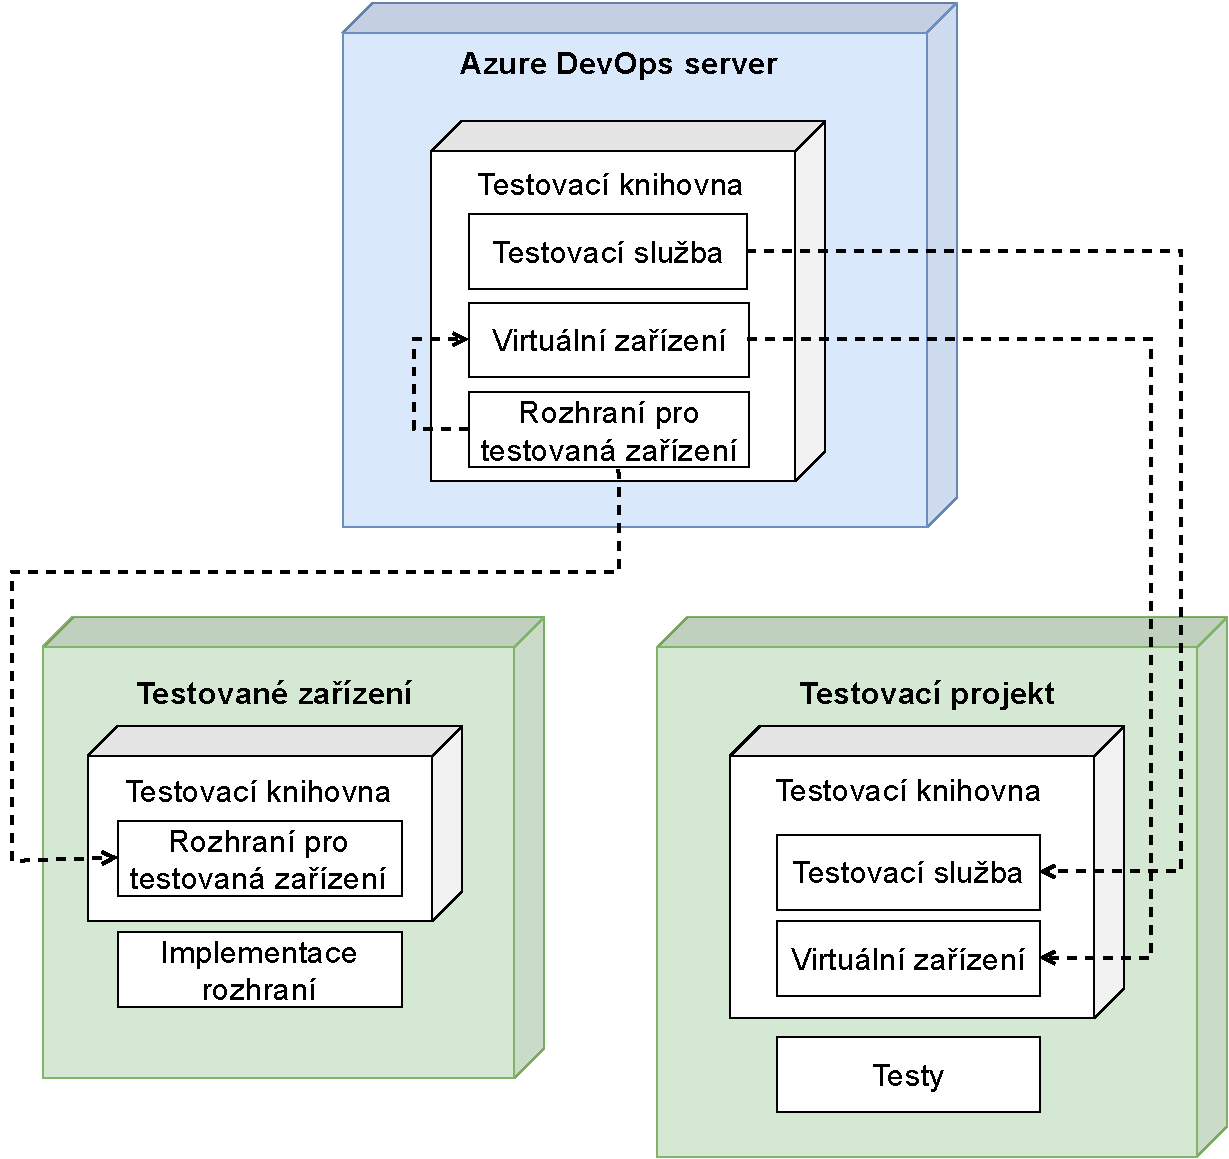
\includegraphics[width=0.75\textwidth]{assets/img/deploymentmodel.pdf}
    \caption{Model distribuce jednotlivých částí knihovny}
    \label{fig:deploymodel}
\end{figure}


\section{Využití průmyslových protokolů}
Jak jsem již definoval v sekci \ref{sec:fieldbus}, protokoly EtherNet/IP a ModbusTCP mají jasně stanovenou komunikaci. Jejich implementace avšak ale není triviální. Z tohoto důvodu je tedy vhodné využít již vytvořené open-source knihovny, které implementují tyto protokoly. V sekcích ukáži vhodné knihovny, které můžou být využity v testovací knihovně.

\subsection{Průzkum open-source knihoven}
K tomu abych mohl správně ohodnotit dostupné open-source knihovny je potřeba definovat kritéria, které musí knihovna splňovat. Jednotlivé knihovny musí být kompatibilní s vytvořenou testovací knihovnou. Tedy, knihovny by měli být implementovány v jazyce \csharp{} a kompatibilní s .NET Framework 4.8. 

Vybrané knihovny budu hodnotit na základě několika faktorů. Mezi tyto faktory bude patřit:

\begin{itemize}
    \item Datum poslední aktualizace
    \item Náročnost využití knihovny, tedy náročnost implementace do knihovny a náročnost následného použití knihovny, hodnocené na stupnici 1--10, kde 1 značí nejjednodušší a 10 nejtěžší 
    \item Hodnocení dokumentace na stupnici 0--10, kde 0 značí, že knihovna neobsahuje žádnou dokumentaci a 10 značí nejkvalitnější dokumentaci
\end{itemize}

Následně na základě těchto kritérií a mém osobním názoru doporučím knihovnu vhodnou k použití s testovací knihovnou. 

\subsubsection{ModbusTCP}

V tabulce \ref{tab:modbus} můžeme vidět seznam nejvhodnějších knihoven pro využití v knihovně. Dle jednotlivých hodnocení můžeme vidět že knihovny se pohybují okolo stejné náročnosti na využití v knihovně. Všechny knihovny jsou dostupné jako NuGet balíčky, což jejich implementaci velice usnadňuje.

Nejpoužívanější knihovnou, dle počtu stažení NuGet balíčku, je knihovna NModbus. Knihovna má průměrnou dokumentaci, kde popisuje jednotlivé třídy. Tato knihovna je udržována komunitně, a již dvakrát byla opuštěna předchozími autory. V kontextu toho, že knihovna má nejstarší datum poslední aktualizace, zde vzniká otázka, zda knihovna bude v budoucnu udržována.

Stejně jako knihovna NModbus, knihovny FluentModbus a Modbus jsou komunitním projektem. Knihovna Modbus ale bohužel neobsahuje žádnou dokumentaci až na krátkou ukázku kódu. Proto má knihovna v hodnocení zvýšenou náročnost na využití kvůli chybějící dokumentaci. Oproti tomu knihovna FluentModbus obsahuje nejlepší dokumentaci ze všech zmíněných knihoven. Bohužel knihovna FluentModbus aktuálně nepodporuje všechny funkce protokolu ModbusTCP. 

Jako nejvhodnější knihovnu jsem tedy vyhodnotil knihovnu EasyModbusTCP. Tato knihovna jako jediná je vytvořena firmou Rossmann Engineering. Z tohoto důvodu předpokládám, že na knihovnu jsou vyvíjeny vyšší kvalitativní nároky, než na ostatní knihovny.  

\begin{table}[H]\centering
    \resizebox{\textwidth}{!}{
        \begin{tabular}{|C{3cm}|C{3cm}|C{2.1cm}|C{1.8cm}|C{2.3cm}|C{4cm}|}\hline
            Název & Autor & Poslední aktualizace & Náročnost využití & Hodnocení dokumentace &  Dostupné na adrese \\\hline 
            EasyModbusTCP & Rossmann Engineering & 04.01.2021 & 1 & 5 & \url{www.easymodbustcp.net}\\\hline
            FluentModbus & Apollo3zehn, et al. & 13.04.2021 & 1 & 6 & \url{www.github.com/Apollo3zehn/FluentModbus} \\\hline 
            NModbus & Rich Quackenbush, et al. & 14.07.2020 & 2 & 4 & \url{www.github.com/NModbus/NModbus} \\\hline 
            Modbus & Andres Müller, et al. & 13.04.2021 & 3 & 1 & \url{www.github.com/AndreasAmMueller/Modbus} \\\hline
        \end{tabular}
    }
    \caption{Seznam dostupných knihoven pro protokol ModbusTCP}
    \label{tab:modbus}
\end{table}

\subsubsection{EtherNet/IP}
Dostupných knihoven pro protokol EtherNet/IP je méně, než pro protokol ModbusTCP. Výhodou opět je, že všechny knihovny jsou koncipovány jako NuGet balíčky. Knihovny EthernetIP a Incore bohužel neobsahují žádnou dokumentaci a obě obdrželi poslední aktualizaci v roce 2018. Náročnost využití je tedy kvůli chybějící dokumentaci proto výrazně zvýšena.

Knihovna EEIP vytvořena opět od firmy Rossmann Engineering. Jako jediná obsahuje kvalitní dokumentaci s ukázkami použití knihovny. Tuto knihovnu jsem vyhodnotil jako nejvhodnější k použití v testovací knihovně.

\begin{table}[htbp]\centering
    \resizebox{\textwidth}{!}{
        \begin{tabular}{|C{3cm}|C{3cm}|C{2.1cm}|C{1.8cm}|C{2.3cm}|C{4.7cm}|}\hline
            Název & Autor & Poslední aktualizace & Náročnost využití & Hodnocení dokumentace &  Dostupné na adrese \\\hline 
            EEIP & Rossmann Engineering & 22.05.2020 & 1 & 5 & \url{www.eeip-library.de/}\\\hline
            EthernetIP & SecondShiftEngineer & 	07.03.2018 & 4 & 0 & \url{www.nuget.org/packages/EthernetIP/} \\\hline
            Incore & Yanjun Wang & 	06.12.2018 & 4 & 0 & \url{www.nuget.org/packages/inc.protocols.ethernetip/}\\\hline
        \end{tabular}
    }
    \caption{Seznam dostupných knihoven pro protokol EtherNet/IP}
    \label{tab:ethernet}
\end{table}